
% This LaTeX was auto-generated from MATLAB code.
% To make changes, update the MATLAB code and republish this document.

\documentclass{article}
\usepackage{graphicx}
\usepackage{color}
\pdfminorversion=7

\title{Lab 04 Report}
\date{2021-04-09}
\author{Christian A. Hardy}

\sloppy
\definecolor{lightgray}{gray}{0.5}
\setlength{\parindent}{0pt}

\begin{document}
\maketitle
  \pagenumbering{gobble}
  \newpage
  
  \pagenumbering{arabic}  
    
\subsection*{Contents}

\begin{itemize}
\setlength{\itemsep}{-1ex}
   \item Experiment 01: Plot Raw Data vs Time
   \item 01 Questions and Answers
   \item Experiment 02: Plot Raw Data vs Time
   \item Experiment 02: Plot LowPass Filtered Data vs Time
   \item 02 Questions and Answers
\end{itemize}


\subsection*{Experiment 01: Plot Raw Data vs Time}

\begin{par}
Using the ismax function with a minimum value trigger of 65 yields mixed results for the heart rate. With the original blue signal, it does not do that much better at getting the actual heart rate versus manually counting portions of the graph. \\

Having a more dynamic system or a more programatic way of determining a threshold would be good for calculating the proper heart rate from this data. I imagine that is what goes into the medical versions of such devices. Accuracy and decent precision is everything afterall. \\

I think a better signal processing algorithm would be more suited normalising the graph. When the signal is particularly amplitude modulated this simple method a finding the heart rate fails more often than not.
\end{par}

    


    \vspace{2em}
\includegraphics [width=4in]{Lab04_01.eps}
\begin{verbatim} Chest Lying Down Heart Rate: 72 \end{verbatim}

\vspace{2em}
\includegraphics [width=4in]{Lab04_02.eps}
\begin{verbatim} Hand Lying Down Heart Rate: 62 \end{verbatim}

\subsection*{01 Questions and Answers}

\begin{par}
Was there variability between the beats? Would you expect the interval between beats to be identical? Why or why not?

\vspace{1em}
There was variability between the beats. This makes sense as the distance from
the heart was different. I would expect the variability between beats to be
extremely close however. Assuming a healthy blood vessel system, then I
couldn't imagine any issues with the

\end{par} \vspace{1em}

\subsection*{Experiment 02: Plot Raw Data vs Time}

    
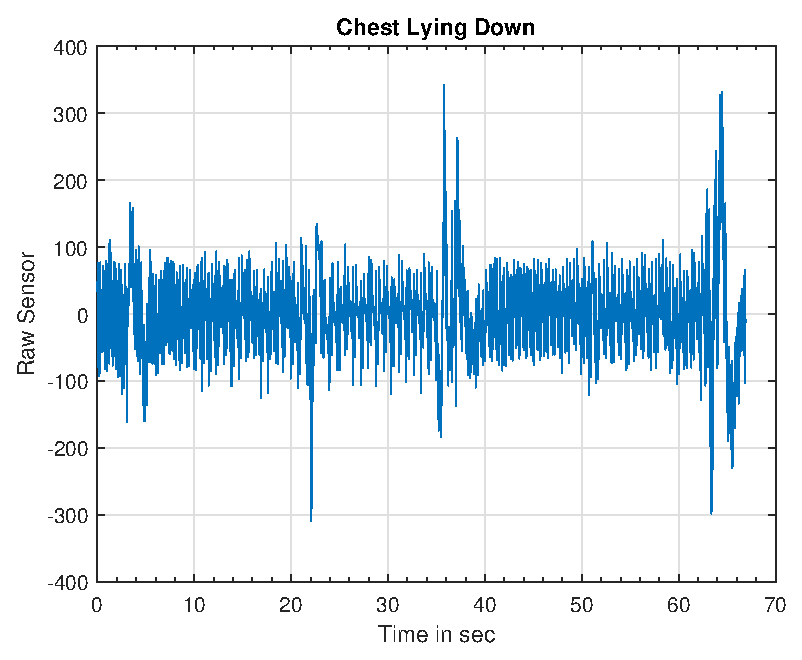
\includegraphics [width=4in]{Lab04_03.eps}
Chest Lying Down Heart Rate:
31
    
\vspace{2em}
\includegraphics [width=4in]{Lab04_04.eps}
Chest Running in Place Heart Rate:
40
    

\vspace{2em}
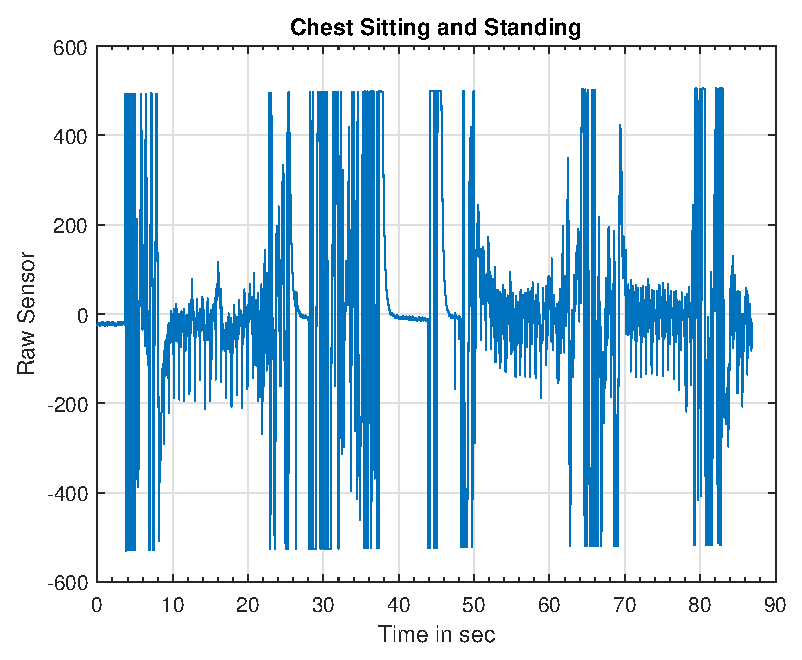
\includegraphics [width=4in]{Lab04_05.eps}
Chest Sitting and Standing Heart Rate:
21
    

\vspace{2em}
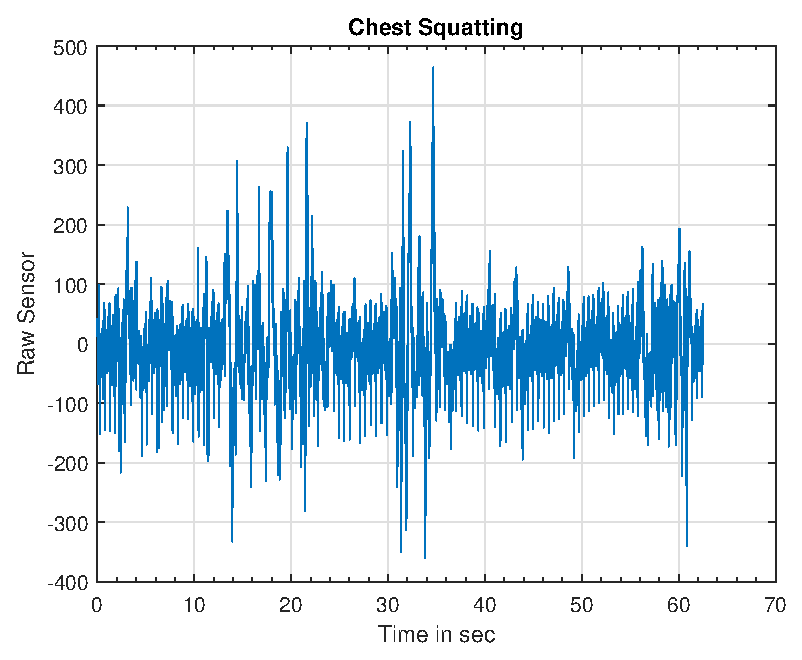
\includegraphics [width=4in]{Lab04_06.eps}
Chest Squatting Heart Rate:
39
    
\vspace{2em}
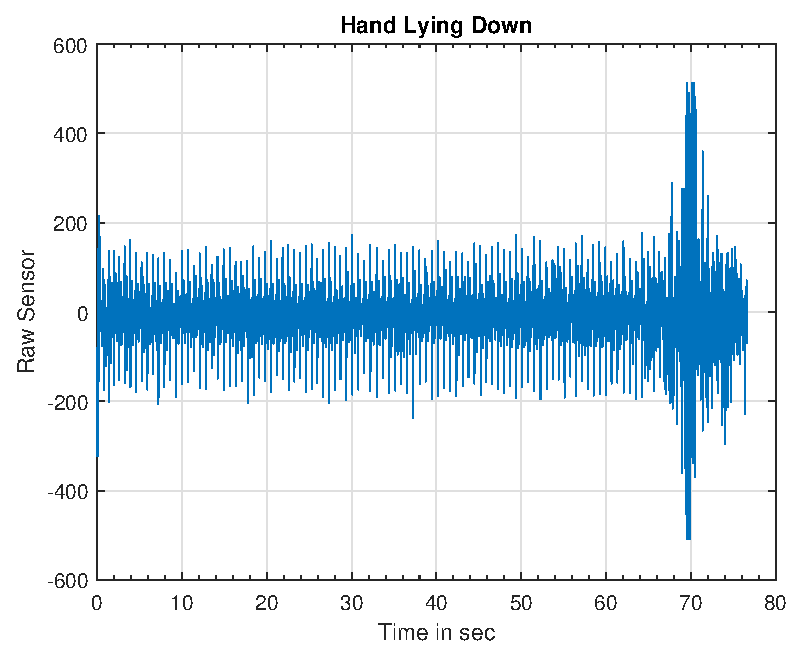
\includegraphics [width=4in]{Lab04_07.eps}
Hand Lying Down Heart Rate:
62

\vspace{2em}
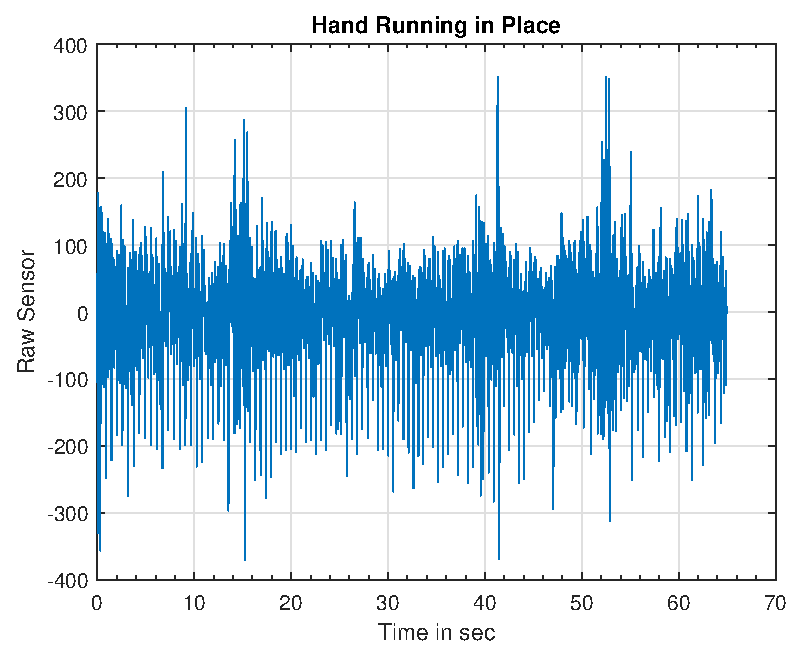
\includegraphics [width=4in]{Lab04_08.eps}
Hand Running in Place Heart Rate:
100

\vspace{2em}
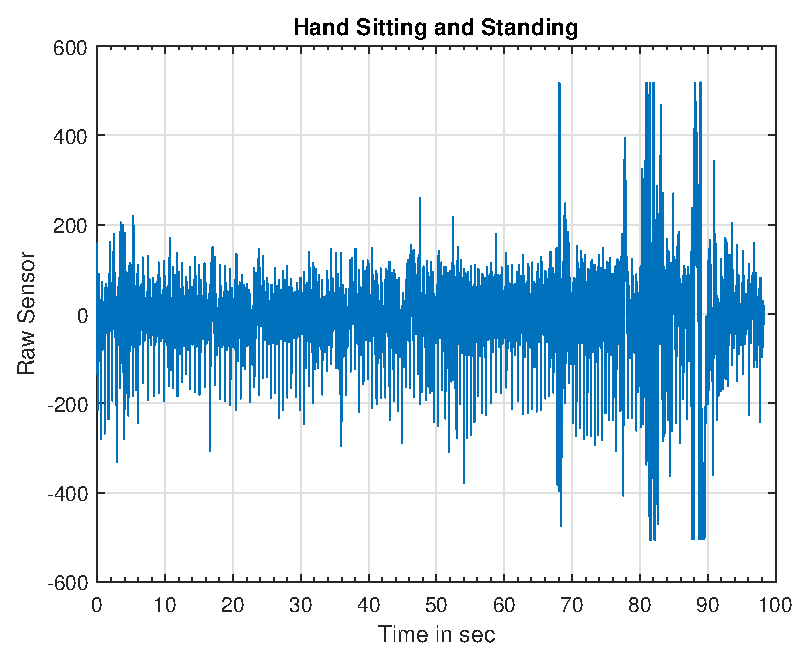
\includegraphics [width=4in]{Lab04_09.eps}
Hand Sitting and Standing Heart Rate:
83

\vspace{2em}
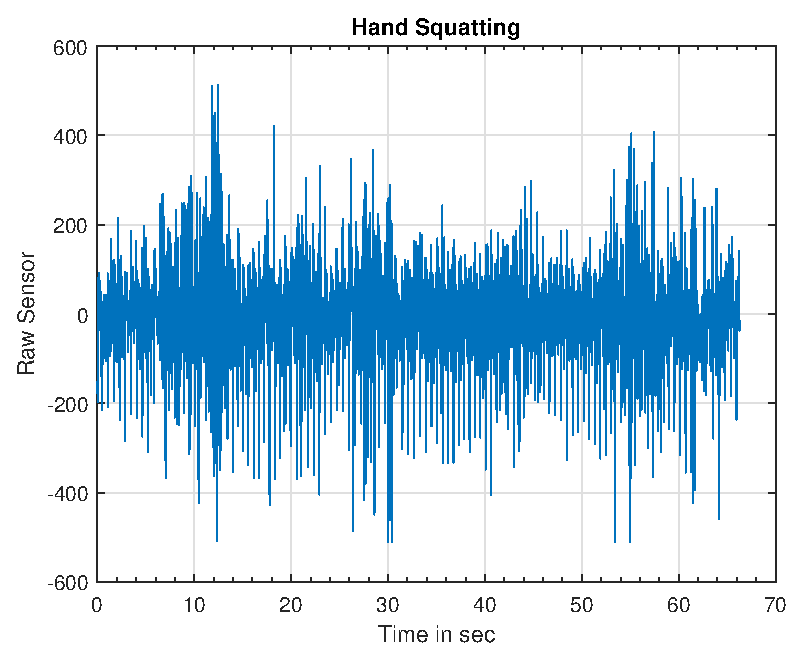
\includegraphics [width=4in]{Lab04_10.eps}
Hand Squatting Heart Rate:
108

\subsection*{Experiment 02: Plot LowPass Filtered Data vs Time}

\begin{par}
Using the ismax function with a minimum value trigger of 65 yields mixed results for the heartrate. Even with the lowpass filtering applied to the signal, shown in red over the original blue signal, it does not do that much better at getting the actual heartrate when manually counting portions of the graph.
\\
Having a more dynamic system or a more programatic way of determining a threshold would be good for calculating the proper heart rate from this data. I imagine that is what goes into the medical versions of such devices. Accuracy and decent precision is everything afterall.
 \end{par} \vspace{1em}
    
\includegraphics [width=4in]{Lab04_11.eps} \begin{verbatim}
Chest Lying Down Heart Rate: 31\end{verbatim} \color{black}

\vspace{2em}
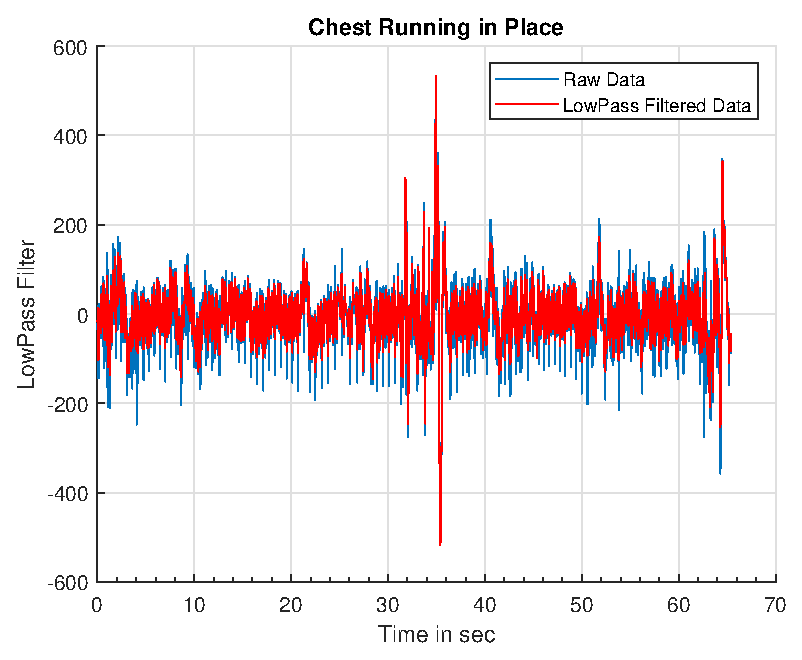
\includegraphics [width=4in]{Lab04_12.eps}  \begin{verbatim}
Chest Running in Place Heart Rate: 40\end{verbatim} \color{black}

\vspace{2em}
\includegraphics [width=4in]{Lab04_13.eps}  \begin{verbatim}
Chest Sitting and Standing Heart Rate: 21\end{verbatim} \color{black}
    
\vspace{2em}
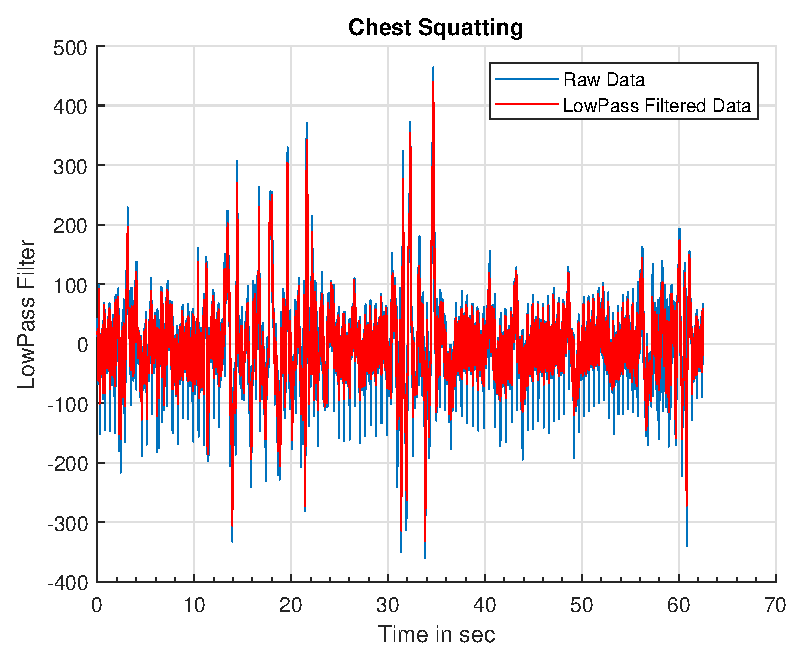
\includegraphics [width=4in]{Lab04_14.eps} \begin{verbatim}
Chest Squatting Heart Rate: 39\end{verbatim} \color{black}

\vspace{2em}
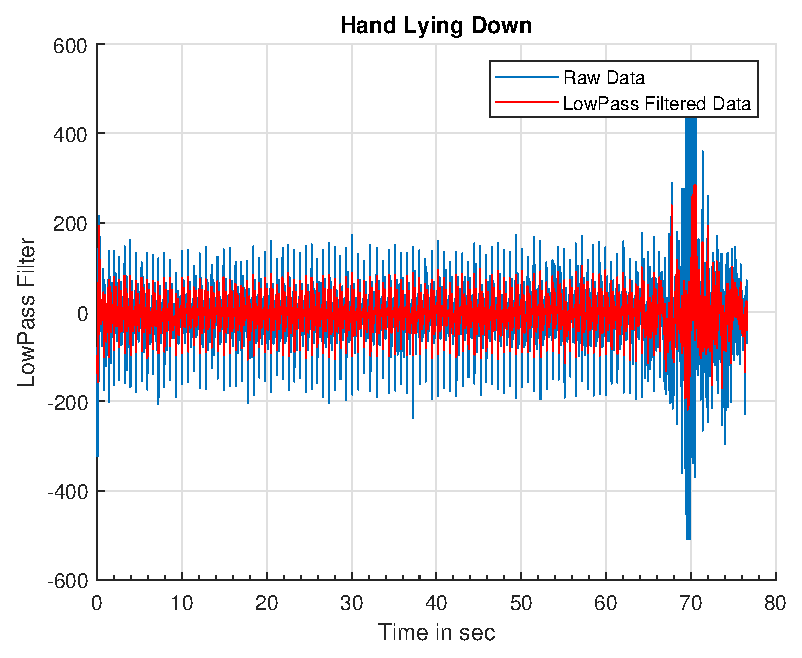
\includegraphics [width=4in]{Lab04_15.eps}  \begin{verbatim}
Hand Lying Down Heart Rate: 62\end{verbatim} \color{black}

\vspace{2em}
\includegraphics [width=4in]{Lab04_16.eps}  \begin{verbatim}
Hand Running in Place Heart Rate: 100\end{verbatim} \color{black}

\vspace{2em}
\includegraphics [width=4in]{Lab04_17.eps}  \begin{verbatim}
Hand Sitting and Standing Heart Rate: 83\end{verbatim} \color{black}

\vspace{2em}
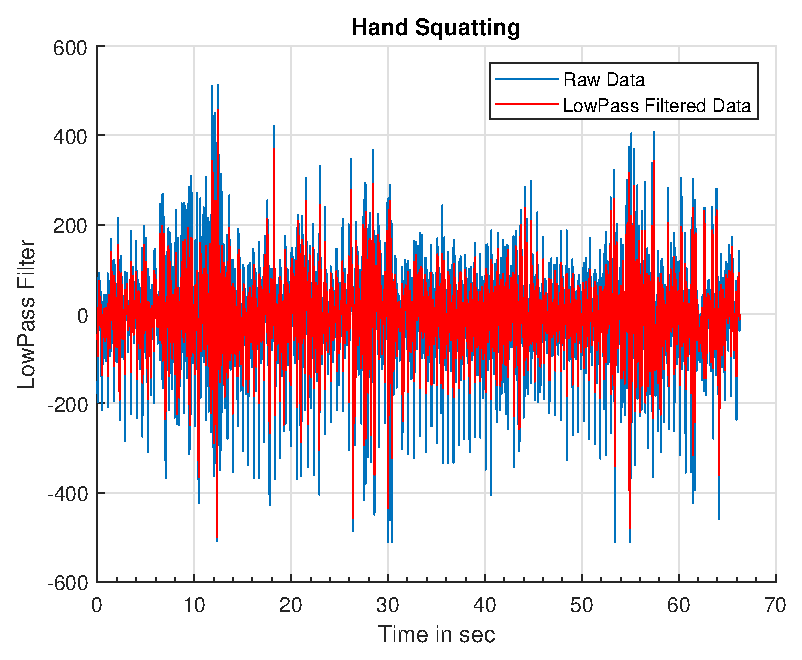
\includegraphics [width=4in]{Lab04_18.eps}  \begin{verbatim}
Hand Squatting Heart Rate: 108\end{verbatim} \color{black}

\subsection*{02 Questions and Answers}

\begin{par}
What physiological advantage is there in a slower resting heart rate?

\vspace{1em}
A slower resting heart rate means your heart is more efficient at pumping
oxengentated blood around your body. Since it is stronger, it pumps less
often, causing less wear on the heart over the lifetime of the person. Also it
likely means that the heart can recover from high periods of activity faster,
returning to a lower rate and easing the workload much faster than a not as
healthy heart.
\end{par}

\end{document}